\documentclass[00_complete]{subfiles}

%\documentclass[12pt]{report}
\usepackage[utf8]{inputenc}
\usepackage{amsmath,amssymb,amsthm,gensymb,parskip,graphicx,footmisc,csquotes,enumerate,datetime2}
\usepackage[]{libertinus}
\usepackage[breaklinks]{hyperref}
\hypersetup{
  pdfauthor={Moshe Krumbein},
  colorlinks=true,
  linkcolor={black},
  filecolor={black},
  citecolor={black}, %blue
  urlcolor={black}, %blue
}
\usepackage[top=30mm,bottom=30mm,left=30mm,right=30mm]{geometry}
%\setlength{\emergencystretch}{2em} % prevent overfull lines
\providecommand{\tightlist}{%
\setlength{\itemsep}{0pt}\setlength{\parskip}{0pt}}

\renewcommand\qedsymbol{$\blacksquare$}

\theoremstyle{definition}
\newtheorem*{definition}{Definition}
\newtheorem*{theorem}{Theorem}
\newtheorem*{axiom}{Axiom}
\newtheorem*{lemma}{Lemma}

\theoremstyle{remark}
\newtheorem*{note}{Note}
\newtheorem*{symbols}{Symbol}
\newtheorem{example}{Example}[section]
\newtheorem*{claim}{Claim}
\newtheorem*{conclusion}{Conclusion}
\newtheorem*{reminder}{Reminder}

\usepackage{fancyhdr}
\usepackage[italicdiff]{physics}
\MakeOuterQuote{"}

\renewcommand{\chaptermark}[1]{\markboth{#1}{}}

\pagestyle{fancy}

\setlength{\headheight}{14.5pt}
\addtolength{\topmargin}{-2.5pt}

\fancyhf{}
\rhead{Moshe Krumbein}
\lhead{\chaptermark}
\cfoot{\thepage}
\fancyhead[R]{\chaptername~\thechapter}
\fancyhead[L]{\mbox{\leftmark}}

\usepackage[Rejne]{fncychap}
\usepackage{titling}

\makeatletter
\renewcommand{\@chapapp}{\vspace*{-100pt}\huge\thetitle}
\makeatother

\makeatletter
\newcommand{\subtitle}[1]{%
  {\center\vspace*{-60pt}%
  \linespread{1.1}\Large\scshape#1%
  \par\nobreak\vspace*{35pt}}
}
\makeatother

\newcommand{\Chapter}[2]{
    \def\n{#2}
    \setcounter{chapter}{\the\numexpr\n-1}
    \chapter{#1}
    \subtitle{\theauthor~- \thedate}
}

\DeclareMathOperator{\Ima}{Im}
\DeclareMathOperator{\Id}{Id}
\DeclareMathOperator{\cis}{cis}

\newcommand{\Mod}[1]{\ (\mathrm{mod}\ #1)}
\newcommand{\st}[0]{\;\mathrm{s.t.}\;}

\title{Discrete Mathematics}
\author{Moshe Krumbein}
\date{Fall 2021}

\begin{document}
\Chapter{Recurrence Relations and Catalan Numbers}{9}

\section{Recurrence Relation}
\begin{definition}[Recursion]
    Sequence $a_n$ is defined as \emph{recursive} if there exists a function $f$
    such that for all $2 \leq n \in \mathbb{N}$:
    $$a_n=\underbrace{f(a_1,a_2,\dots, a_{n-1})}_{\text{recurrence relation}}$$
\end{definition}
\begin{definition}[Recurrence Relation]
    We say that $a_n$ is defined as a \emph{recurrence relation} of order $k$
    if for all $n>k$:
    $$a_n=f(a_{n-1},a_{n-2,\dots,a_{n-k}})$$
\end{definition}
\begin{example}[Arithmetic Progression]
\begin{gather*}
    a_1=a \\
    \forall n \geq 2 \quad a_n = a_{n-1}+d,d \in \mathbb{R} \\
    a_n = a+ (n-1)d
\end{gather*}
\end{example}
\begin{example}[Geometric Progression]
\begin{gather*}
    a_1=a \\
    \forall n \geq 2 \quad a_n = a_{n-1} \cdot q \\
    a_n = aq^{n-1}
\end{gather*}
\end{example}
\begin{example}[Tower of Hanoi]
    What are the minimum number of a steps to move a tower of height $n$ to the rightmost
    place?

    \begin{figure}[ht]
  \centering
    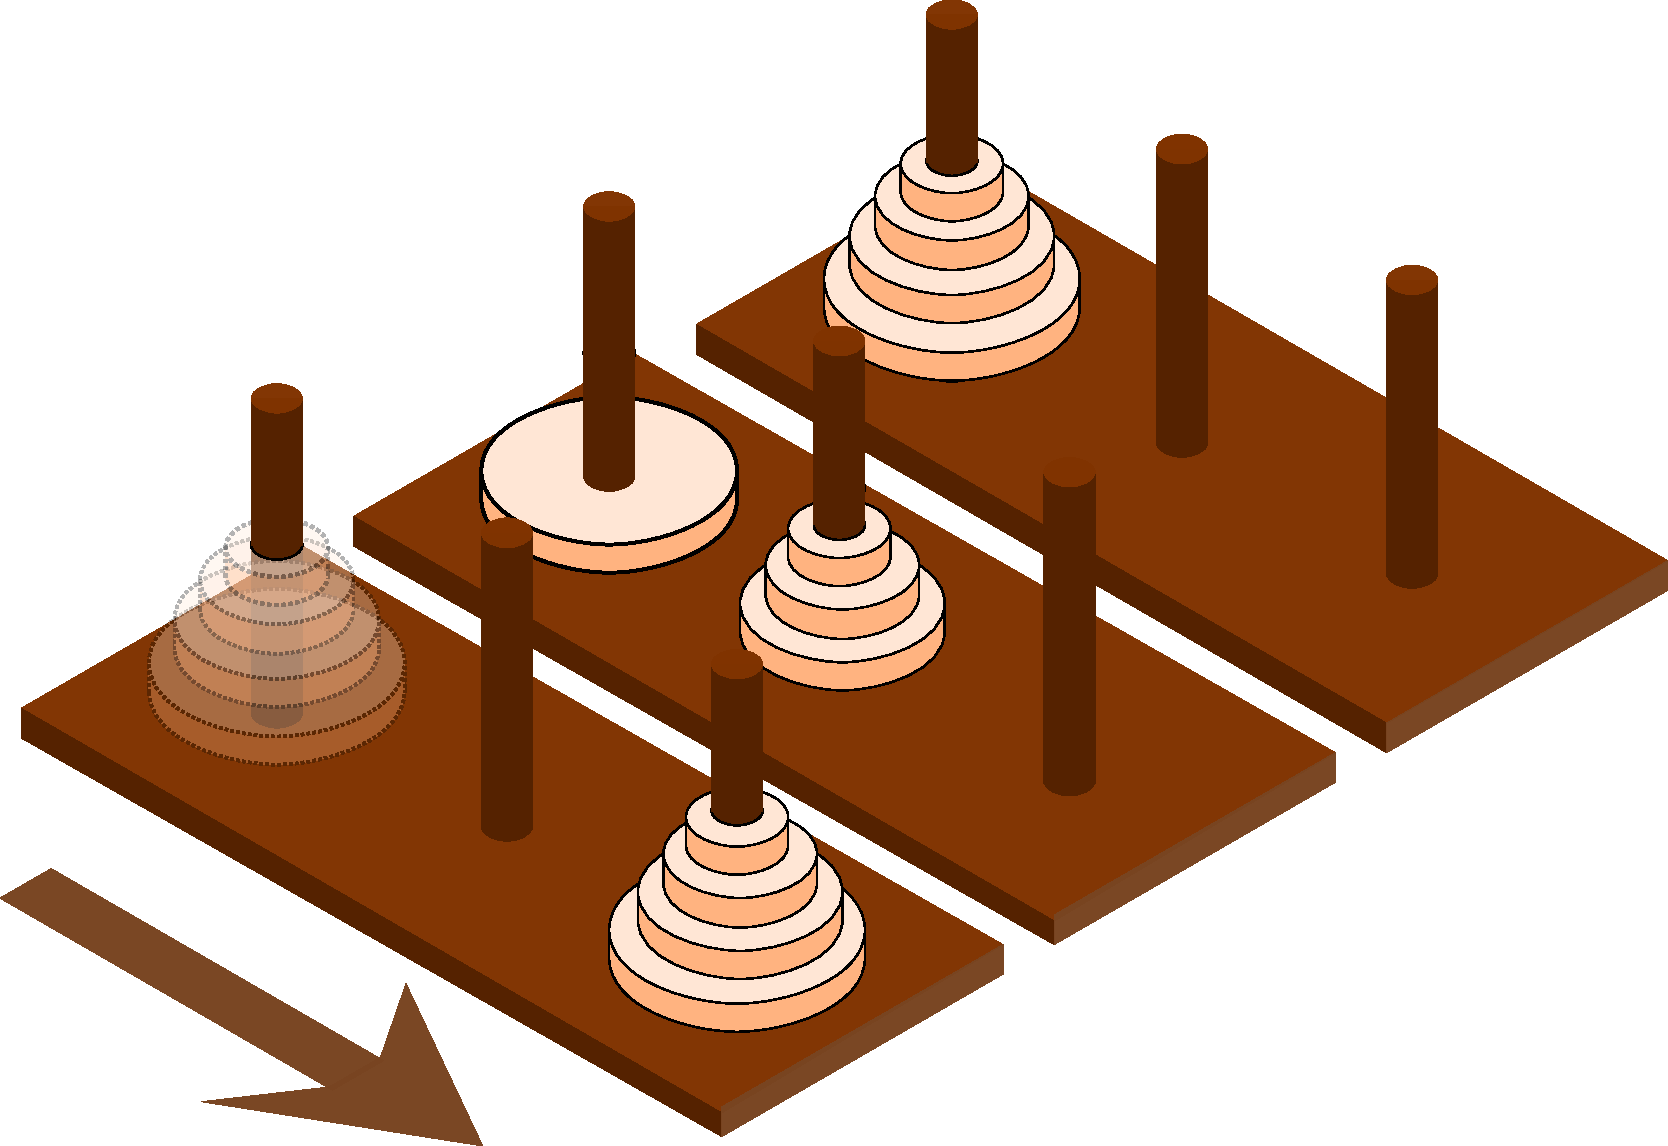
\includegraphics[width=0.5\textwidth]{w8-tower}
    \caption{Tower of Hanoi}
\end{figure}

    Base case: $a_1=1$.

    In order to move the $n$th ring, we first have to move $n-1$ rings to the
    middle, move the $n$th ring, and then to move back all then $n-1$ rings.
    $$a_n=2a_{n-1}+1$$
    We see that $a_2=3$ and $a_3=7$. Maybe $a_n = 2^n-1$?
    \begin{proof}
    Let us check using induction:
    \begin{enumerate}[I.]
        \item \begin{equation}
            a_1=1 \tag{\checkmark}
        \end{equation}
        \item \begin{equation}
            a_n = 2a_{n-1}+1=2\cdot(2^{n-1}-1)+1=2^n-2+1=2^n-1
            \tag{\checkmark}
        \end{equation}
    \end{enumerate}
    \end{proof}
\end{example}
\begin{example}[Fibonacci Sequences]
    We have two newly-born rabbits.
\begin{itemize}
    \item After a month of being born they become mature
        \item After a month of maturity they will give birth to a pair of baby
            bunnies
        \item Rabbits do not die.
\end{itemize}
\begin{gather*}
    f(0)=1, f(1)=1, f(2)=2, f(3)=3
\end{gather*}
Recurrence sequence (of order $2$):
$$f(n)=\underbrace{f(n-2)}_{\text{just born}}+\underbrace{f(n-1)}_{\text{old
rabbits}}$$
\begin{symbols}
    $$\varphi = \frac{1+\sqrt 5}{2} \qquad \overline \varphi = \frac{ 1- \sqrt 5}{2}$$
    When are the solution to the following equation:
    $$x^2=x+1$$
\end{symbols}
\begin{claim}
    For all $n \in \mathbb{R}\cup\{0\}$:
    \begin{gather*}
        f(n)=\frac{1}{\sqrt 5}\left(\varphi^{n+1}-\overline \varphi^{n+1}\right)
        =\frac{1}{\sqrt 5}\left(\left(\frac{1+\sqrt 5}{2}\right)^{n+1}-\left(\frac{1-\sqrt 5}{2}\right)^{n+1}\right)
    \end{gather*}
\end{claim}
\begin{proof}
    Using induction:
    \begin{enumerate}[I.]
        \item \begin{equation}
            f(0)=1, \quad f(1)=1
            \tag{\checkmark}
        \end{equation}
        \item
        \begin{gather*}
            f(n+1)=f(n)+f(n-1)=\frac{1}{\sqrt 5}(\varphi^{n+1}-\overline
            \varphi^{n+1}+\varphi^n-\overline \varphi^n) \\
            = \frac{1}{\sqrt 5} (\varphi^n(\varphi+1)-\overline
            \varphi^n(\overline \varphi +1)) \\
            =\frac{1}{\sqrt 5}(\varphi^n\varphi^2-\overline \varphi^n \overline
            \varphi^2) = \frac{1}{\sqrt 5}(\varphi^{n+2}-\overline \varphi^{n+2})
            \tag{\checkmark}
        \end{gather*}
    \end{enumerate}
\end{proof}
\end{example}
\begin{example}
        We have a ladder with $n$ rungs. In every step we can go up one
        or two rungs.

        $J(n)$ is the number of ways to up a ladder with $n$ rungs.
        \begin{gather*}
        J(1)=1, \quad J(2)=2, \quad J(3)=3 \\
        J(n) =
        \underbrace{J(n-1)}_{\text{the last step is to go up one rung}}+
        \underbrace{J(n-2)}_{\text{the last step is to go up two rungs}}
        \end{gather*}
        Which is a \emph{Fibonacci sequence} with the initial values of
        $J(1)=1, J(2)=2$.
\end{example}
\begin{example}
    $g(n)$ is defined as the number of subsets of the set $\{1,\dots,n\}$ that do not contain two
    consecutive numbers.

    Essentially, this is another \emph{Fibonacci sequence} with the initial
    values $g(0)=1,g(1)=2$.
\end{example}
\section{Catalan numbers}
\begin{definition}[Catalan numbers]
    We define $C(n)$ as the number of paths on the grid from $(0,0)$ to $(n,n)$
    that do not cross the line $y=x$.
    $$C(n)=\frac{1}{n+1}\binom{2n}{n}$$
\end{definition}
Let us build a recursive definition for $C(n)$.

First, we see that our first step must be a step to the right and our last step
must be a step up (this is obvious because we have already proved that the
function is \emph{invertible}). ($C(0)=1$)

We define for all $1 \leq i \leq n$ set $A_i$ as the number of paths from
$(0,0)$ to $(n,n)$ such that the first time we touch the line $y=x$ is at the
point $(i,i)$. Based on this we see:
$$\bigcup_{i=1}^n|A_i| = C(n)$$

The size of $A_i$ can be defined as the number of legal paths from $(0,0)$ until
$(i,i)$ \emph{without} touching $y=x$, which is essentially shifting our line
to $y=x-1$ ($C(i-1)$), times the number of legal paths from $(i,i)$ to $(n,n)$
($C(n-i)$).
$$|A_i|=C(i-1) \cdot C(n-i)$$
In conslusion, we receive the following \emph{recurrence sequence}:
$$C(n) = \sum_{i=1}^{n}C(i-1)\cdot C(n-i)$$

\begin{example}
Thirding a polygon is done by going over all the diagonals that don't
cross over each other.

How many ways are there to "third" a given polygon?

We symbolize with $a_n$ the number of ways we can divide a polygon with
$n+2$ sides into three parts.
$$a_1=1 \qquad a_2=2$$

We define $A$ to be all of the ways we can divide the polygon into thirds:

\begin{itemize}
    \item[$A_1$ -] Set of all the thirds that contain the triangle
        $\{1,n+1,n+2\}$

    $|A_1|=a_{n-1}$
    \item[$A_2$ -] Set of all the thirds that contain the triangle
        $\{2,n+1,n+2\}$

    $|A_1|=a_{1}a_{n-2}$
\end{itemize}
For all $1 \leq k \leq n$, we define:
\begin{itemize}
    \item[$A_k$ -] Set of all the thirds that contain the triangle
        $\{k,n+1,n+2\}$
\end{itemize}
$$A=\bigcup_{k=1}^n A_k \implies a_n =|A|=|A_1|+|A_2|+\dots+|A_n|$$
We will now find the size of $A_k$: each thirding in $A_k$ divides the
polygon into three parts: the triangle
$\underbrace{\{k,n+1,n+2\}}_{\text{number of thirds}-1}$, the polygon
$\underbrace{\{1,2,4,\dots,k,n+1\}}_{\text{number of thirds}-a_{k-1}}$ and the
polygon $\underbrace{\{k,k+1,\dots,n+1\}}_{\text{number of thirds}-a_{n-k}}$.

$$|A_k|=a_{k-1}a_{n-k}$$
\begin{conclusion}
    \begin{gather*}
        a_n=\sum_{k=1}^{n}|A_k|=\sum_{k=1}^{n}a_{k-1}a_{n-k} \\
        a_1 = 1 \qquad a_0 = 1
    \end{gather*}
    We see that this is exactly like the Catalan numbers:
    \begin{gather*}
        a_1=c(1) \qquad a_0=c(0) \\
        a_n=c(n) \\
        \boxed{a_n=\frac{1}{n+1}\binom{2n}{n}}
    \end{gather*}
\end{conclusion}
\end{example}
\end{document}
